
% Homework template for MA 614, Spring 2011.  When a line begins with the percent sign, the typesetter ignores it.  So, use percent signs at the beginning of lines to insert comments to yourself.


% Set the document class.  The command [11pt] sets the font at 11 point, which is nicer to read.  The default would be 10pt
\documentclass[11pt]{amsart} 


% Call packages that allow you to invoke certain mathematical symbols.
\usepackage{amssymb,amsmath,amsthm}
\usepackage[framed,numbered,autolinebreaks,useliterate]{mcode}
\usepackage{graphicx}
\usepackage{natbib}
% Set the title, author, and date information.
\title{EE 523: Homework 1}
\author{Anil A. Aksu}
\date{\today}


% Formally begin the document and make the title.
\begin{document}
\maketitle

\section*{Problem 1 }

Maxwell equations are given as\cite{Cheng}: 
\begin{equation}
\label{eq:1}
\mathbf{\nabla}\cdot \mathbf{D}=\rho,
\end{equation}
\begin{equation}
\label{eq:2}
\mathbf{\nabla}\times \mathbf{E}=-\frac{\partial \mathbf{B}}{\partial t},
\end{equation}
\begin{equation}
\label{eq:3}
\mathbf{\nabla}\cdot \mathbf{B}=0,
\end{equation}
\begin{equation}
\label{eq:4}
 \mathbf{\nabla}\times \mathbf{H}=\mathbf{J}+\frac{\partial \mathbf{D}}{\partial t}.
\end{equation}
Note that $\mathbf{D}= \epsilon \mathbf{E}$ where $\epsilon$ is the permittivity of free space, $\mathbf{H}=\mu \mathbf{B}$ where $\mu$ is permeability of free space and $J=\rho \mathbf{v}$ where $\mathbf{v}$ is the charge velocity. By using Maxwell equations given above, show that proper boundary conditions between two media with permittivities  $\epsilon_1,\epsilon_2$, permeabilities $\mu_1,\mu_2$ separated with an interface with unit normal $\mathbf{a}_{n}$ can be given as\cite{Cheng,Hesthaven2001}:
\begin{equation*}
D_{1n}-D_{2n}=\rho_s,
\end{equation*}
\begin{equation*}
E_{1t}=E_{2t},
\end{equation*}
\begin{equation*}
B_{1n}=B_{2n},
\end{equation*}
\begin{equation*}
\mathbf{a}_{n}\times(\mathbf{H}_{1}-\mathbf{H}_{2})=\mathbf{J}_s.
\end{equation*}
where $n$ and $t$ subscripts stand for normal and tangential components of the vector field, $s$ subscript stands for quantities at the surface.
\\
\textbf{Solution:}\\
The volume integral of equation \ref{eq:1} covering the interface between two media can be given as:
\begin{equation}
\label{eq:5}
\int_{V_1} \mathbf{\nabla}\cdot \mathbf{D} \mathrm{d} V + \int_{V_2} \mathbf{\nabla}\cdot \mathbf{D} \mathrm{d} V=\int_{V_1+V_2} \rho \mathrm{d} V.
\end{equation}
As the volume $V_1$ and the volume $V_2$ shrinks to the interface\cite{Chadwick}, the volume integrals at the left hand-side of equation \ref{eq:5} can be given as surface integrals, but the right hand-side of equation \ref{eq:5} still stay as volume integral and converges to the surface charge density as follows:
\begin{equation}
\label{eq:6}
\int_{S} (\mathbf{D}_1 -\mathbf{D}_2) \mathbf{a}_n\mathrm{d}S=\int_{S} \rho_s \mathrm{d}S.
\end{equation}
Therefore, the product of $\mathbf{D}$ with the unit normal of the interface between two media results in the following boundary (interface) condition:
\begin{equation}
D_{1n}-D_{2n}=\rho_s.
\end{equation}

\begin{figure}
\centering
 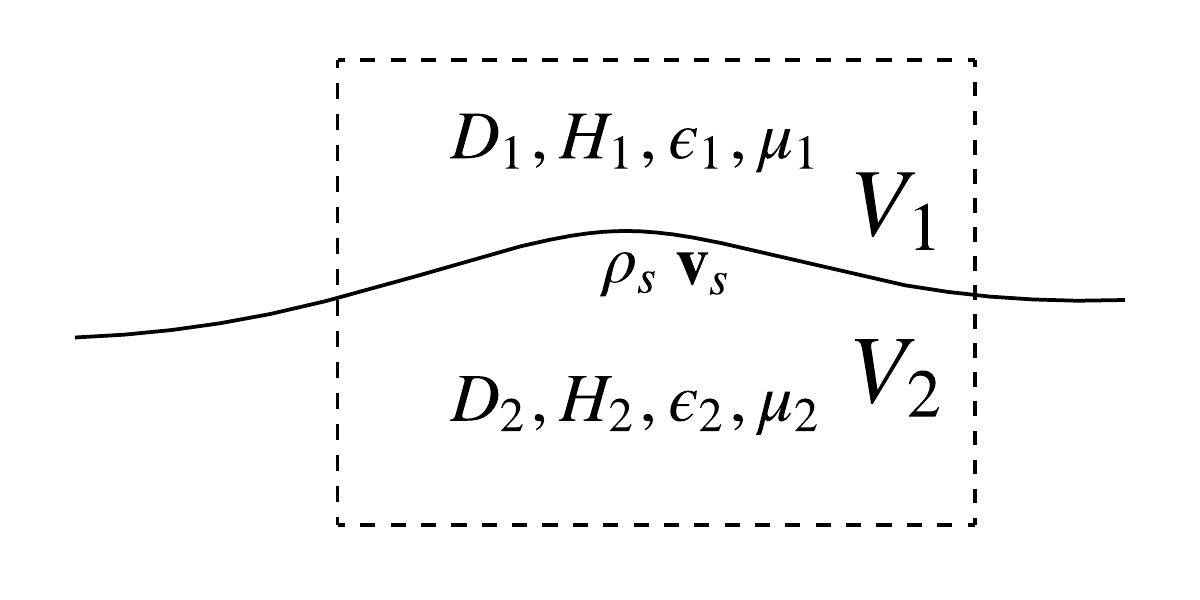
\includegraphics[scale=0.3]{JumpSurface}% Images in 100% size
  \caption{Jump surface separating media with permittivities  $\epsilon_1,\epsilon_2$, permeabilities $\mu_1,\mu_2$. }
\label{fig:Jump}
\end{figure} 

Similarly, equation \ref{eq:2} can be integrated in a volume covering the interface as follows:
\begin{equation}
\label{eq:7}
\int_{V_1} \mathbf{\nabla}\times \mathbf{E} \mathrm{d} V + \int_{V_2} \mathbf{\nabla}\times \mathbf{E} \mathrm{d} V=-\int_{V_1+V_2} \frac{\partial \mathbf{B}}{\partial t} \mathrm{d} V.
\end{equation}
As the volume $V_1$ and the volume $V_2$ shrinks to the interface, the volume integrals at the left hand-side of equation \ref{eq:7} can be given as surface integrals, but the right hand-side of equation \ref{eq:7} still stay as volume integral:
\begin{equation}
\label{eq:8}
\oint_{\partial V_1} \mathbf{\mathbf{a}}\times \mathbf{E} \mathrm{d} S + \oint_{\partial V_2} \mathbf{\mathbf{a}}\times \mathbf{E} \mathrm{d} S=-\int_{V_1+V_2} \frac{\partial \mathbf{B}}{\partial t} \mathrm{d} V.
\end{equation}
The right hand-side of equation \ref{eq:8} becomes negligible as the volume shrinks to the interface, therefore the integral \ref{eq:8} reduces to the following relation:
\begin{equation}
\label{eq:9}
\oint_{\partial V_1} \mathbf{\mathbf{a}}\times \mathbf{E} \mathrm{d} S + \oint_{\partial V_2} \mathbf{\mathbf{a}}\times \mathbf{E} \mathrm{d} S=0
\end{equation}
Equivalently,
\begin{equation}
E_{1t}=E_{2t},
\end{equation}

The volume integral of equation \ref{eq:3} covering the interface between two media can be given as:
\begin{equation}
\label{eq:10}
\int_{V_1} \mathbf{\nabla}\cdot \mathbf{B} \mathrm{d} V + \int_{V_2} \mathbf{\nabla}\cdot \mathbf{B} \mathrm{d} V=0.
\end{equation}
As the volume $V_1$ and the volume $V_2$ shrinks to the interface\cite{Chadwick}, the volume integrals at the left hand-side of equation \ref{eq:10} can be given as surface integrals:
\begin{equation}
\label{eq:11}
\int_{S} (\mathbf{B}_1 -\mathbf{B}_2) \mathbf{a}_n\mathrm{d}S=0.
\end{equation}
Therefore, the product of $\mathbf{D}$ with the unit normal of the interface between two media results in the following boundary (interface) condition:
\begin{equation}
B_{1n}=B_{2n}.
\end{equation}


Finally, equation \ref{eq:4} can be integrated in a volume covering the interface as follows:
\begin{equation}
\label{eq:12}
\int_{V_1} \mathbf{\nabla}\times \mathbf{H} \mathrm{d} V + \int_{V_2} \mathbf{\nabla}\times \mathbf{H} \mathrm{d} V=\int_{V_1+V_2} \mathbf{J} \mathrm{d} V+\int_{V_1+V_2} \frac{\partial \mathbf{D}}{\partial t} \mathrm{d} V.
\end{equation}
As the volume $V_1$ and the volume $V_2$ shrinks to the interface, the volume integrals at the left hand-side of equation \ref{eq:12} can be given as surface integrals, but the right hand-side of equation \ref{eq:12} still stay as volume integral:
\begin{equation}
\label{eq:13}
\oint_{\partial V_1} \mathbf{\mathbf{a}}\times \mathbf{H} \mathrm{d} S + \oint_{\partial V_2} \mathbf{\mathbf{a}}\times \mathbf{H} \mathrm{d} S=\int_{V_1+V_2} \mathbf{J} \mathrm{d} V+\int_{V_1+V_2} \frac{\partial \mathbf{D}}{\partial t} \mathrm{d} V.
\end{equation}
The right hand-side of equation \ref{eq:13} becomes negligible as the volume shrinks to the interface, therefore the integral \ref{eq:13} reduces to the following relation:
\begin{equation}
\label{eq:14}
\oint_{\partial V_1} \mathbf{\mathbf{a}}\times \mathbf{H} \mathrm{d} S + \oint_{\partial V_2} \mathbf{\mathbf{a}}\times \mathbf{H} \mathrm{d} S=\int_{V_1+V_2} \mathbf{J} \mathrm{d} V.
\end{equation}
As a result,
\begin{equation*}
\mathbf{a}_{n}\times(\mathbf{H}_{1}-\mathbf{H}_{2})=\mathbf{J}_s.
\end{equation*}

\bibliographystyle{plain}
% Note the spaces between the initials
\bibliography{EE523}
\end{document}
